\documentclass[10pt]{article}
\usepackage{titling} % Import titles.
% Make page wider so title fits better on the front page.
\usepackage[ 
paperheight  = 297mm, paperwidth  = 210mm,  % or: "paper=a4paper"
layoutheight = 197mm ,layoutwidth  = 130mm,
layoutvoffset = 50mm, layouthoffset = 40mm,
includeheadfoot,
top=-1in, bottom=-1in, left=-1in, right=-1in,
textwidth=20cm
]{geometry}
\usepackage[backend=biber,sorting=none, style=nature]{biblatex}
\addbibresource{Bib_Pathogenicity.bib}
%\usepackage{xr} % Allows to make references across different files, if not by default.
%\externaldocument{Chapters/Variant_Prediction_Genome_Diagnostics}
%\externaldocument{Chapters/Cell_death}
%\externaldocument{Chapters/Monte_Carlo}
%\externaldocument{Chapters/Materials_And_Methods}
%\externaldocument{Chapters/Results}
\usepackage{graphicx} % Import images.
\graphicspath{{./Figures/}} % Set image directory.
\usepackage[hidelinks]{hyperref} % Make table of contents clickable and remove colours in viewer.
\usepackage{siunitx} % Allows the degree symbol in math environments.
\usepackage{enumerate} % Make lists of steps.
\usepackage{caption} % Allows captions in tables and figures.
\usepackage{subcaption} % Allows subfigures.
\usepackage{longtable} % Allows long tables / multipage tables.
\usepackage{pdfpages} % GIves the possibility import pdf pages.

\begin{document}
	\pagenumbering{gobble}
	\title{Protein structure modeling for variant pathogenicity prediction}
	\author{Author: Sylt Schuurmans\\
		Studentnumber: 333332\\
		Study: Bio-informatica\\
		Hanze hogeschool: Institute for Life Science and Technology\\
		Supervisor: Martijn Herber\\
		Hospital: Universitary Medical Center Groningen: Department of Genetics\\
		Supervisor : Joeri van der Velde}
	\maketitle
	\newpage
	
	% Make text width normal.
%	\restoregeometry
	\newgeometry{top=2in,
	bottom=1in,
	left=1in,
	right=1in,
	textwidth=14cm}
	
	\section*{Abstract}
	Around 1 in 17 people is affected by one of ~7,000 known rare diseases. Most of these patients do not receive a diagnosis, which means they remain in uncertainty without a prognosis, are unable join specific patient support groups, and do not receive the most appropriate treatment.
Next-generation sequencing (NGS) of DNA promises to establish a molecular diagnosis and help these patients but many challenges still stand in the way of maximum success.
Recent years have seen great advances in computational tools that quickly reduce the amount of DNA variants to be interpreted by a human expert for potentially pathogenic effects.
But, the current tools that rely on features such as evolutionary conservation, annotation of regulatory genomics elements and structural DNA features have been already optimized over many years and significant improvements are not expected. 
Here we tried to introduced structural features of proteins into diagnostics based on the methods used by VIPUR. Through the difficulties of protein modeling and experts knowledge it was discovered that methods used by VIPUR are not features that can help in diagnosis with machine learning. Structural data of proteins is often incomplete and is highly dependent on experimentally determined structures which are expensive to make. The methods that VIPUR uses to standardize protein structures for machine learning removes the context and treats them like they are in a vacuum. To gain a more realistic view on structural information we chose to use the web service HOPE. We also developed a method to gain insight in the structural features of a protein and several of its variants. With these methods we tried to collect structural information which is usable for diagnosis.
	\label{section:Chap_Introduction}
	\newpage
	
	\section*{Acknowledgment}
	This graduation project has taken place at Universitary Medical Center Groningen (UMCG) at the Department of Genetics within the genomics coordination center (GCC), this report has been written for the GCC to gain insight into structural data to improve the GAVIN variant predictor. I want to thank Joeri van der Velde for supervising me during this project and helping me with writing this report. I also would like to thank Benjamin Kant and Marielle van Gijn for helping me decide to focus on assessing tumor necrosis factor associated receptor-associated periodic syndrome (TRAPS). And I especially would like to thank Tsjerk Wassenaar for informing us about the function and structure of TNFRSF1A, giving us the appropriate protein structures to work with and steering this project into a meaningful direction.
	\newpage
	
	\section*{Abbreviations}
	ACCP Solvent Accessible Surface Area\\
APAF1 Apoptotic Protease Activating Factor\\
API Application Programming Interface\\
Bash Bourne Again Shell\\
CPU Central Processing Unit\\
CSV Comma Seperated Values\\
DNA Deoxyribose Nucleic Acid\\
DISC Death-Inducing Signaling Complex\\
FEM Fixed End Move\\
GAVIN Gene-Aware Variant INterpretation\\
GRCh/hg Genome Reference Consortium Human Human Genome\\
MD	Molecular Dynamics\\
MPI Message Parsing Interface\\
NCBI National Center for Biotechnology Information\\
OS Operating System\\
PDB Protein Data Bank\\
PM Pivot Movement\\
PSI-BLAST Position Specific Iterative BLAST\\
PSSM Position Specific Scoring Matrix\\
RCSB Research Collaboratory for Structural Bioinformatics\\
SASA Solvent Accessible Surface Area\\
SLURM Simple Linux Resource Management\\
TNF Tumor Necrosis Factor\\
TNFRSF1A Tumor Necrosis Factor Receptor Superfamily Member 1A\\
TRAPS Tumor Necrosis Factor Associated Receptor-Associated Periodic Syndrome\\
VIPUR Variant Interpretation Using Rosetta\\
VTS VIPUR Training Set\\
	\label{section:Chap_Abbreviations}
	\newpage
	
	\tableofcontents
	\newpage
	
	\listoffigures
	\newpage
	
	\listoftables
	\newpage
	
	\pagenumbering{arabic}
%	\section[Section Title. Section Subtitle]{Section 
%		Title\\ {\large Section Subtitle}}
	\section[Introduction]{Introduction: Variant prediction in genome diagnostics and the addition of protein modeling}
	Evidence is based on conservation whether it works or not

Telling about the current state of gene variant prediction in the perspective of machine learning, GAVIN, SIFT, CADD


	\label{section:Chap_Variant_Prediction_In_Genome_Diagnostics}
	\newpage
	
	\section{Theory}
	\subsection{A general concept of structural levels within proteins}

The formation of protein structures is classified in different levels, distinctions are made based on bindings and structures that arise from them. 
The order in which amino acids appear in a sequence is called the primary structure, in this level amino acids are only bound to each other by peptide bonds. 
Within a primary structure amino acids can form new peptide bonds between the N and C -terminus of an amino acid, with these bonds 3D structures are made called $\alpha$ helices and $\beta$-sheets that together make up the secondary structure.
More alterations to a single amino acid sequence in the 3D can come from disulfide bridges, ion, hydrogen -bonds, hydrophobic and hydrophilic -interactions formed by the residues of the amino acids, together these bonds form the tertiary structure.
By combining multiple tertiary structures the quaternary structure of a protein can be formed out of the mentioned bonds, bridges and interactions.

\subsection{Problems in protein modeling and strategies for resolving structures}
At the moment of writing more than 158000 \cite{} protein structures have been resolved by experimental methods such a X-ray crystallography and nuclear magnetic resonance (NMR). 
% wwPDB: Deposition Statistics, wwPDB	
Importance of experimental determination instead of just modeling

Modeling protein techniques as homology modeling and protein threading

Simulations such as gromacs 
	\label{section:Chap_PMT}
	\newpage
	
	\subsection{Monte Carlo Method}
There are complex problems in a variety of research fields which could take up years or even centuries to compute with simple deterministic methods. For some problems there is an algorithm which makes it possible to cut down computation time significantly, but when no deterministic algorithm is available to speed up the process an empirical probabilistic method might be able to approximate the desired result. With the Monte Carlo method random samples are taken from the parameter space ,that describe a data set, and fed into a model which produces a potential outcome. By repeating the process more results are generated until at some point the data can display a pattern that describes the outcome. The result is a quantified probability which describes the chance that something might occur based on the quantity of occurrence generated by the model \cite{}.
%Monte Carlo Simulation / Method, Stephanie
%Monte Carlo method, Wikipedia
\newline
\newline
The Monte Carlo methods can differ depending on the algorithm and application in which it is used, but in summary most implementations will follow a general pattern \cite{}:
%Monte Carlo method, Wikipedia
\begin{enumerate}
	\setcounter{enumi}{-1}
	\item Construct a model which is able to describe an outcome of the problem.
	\item Define the space of which inputs can be used by the model to get an outcome (creating a parameter space). 
	\item Use the model to generate results based on random sampled input from the parameter space.
	\item Order and determine which results are part of a certain outcome and draw conclusions on the generated statistical evidence.
\end{enumerate}

\label{subsec:Monte_Carlo_Method}

\subsection{The use of the Monte Carlo method and its pitfalls}
The Monte Carlo method has a limited scope of problems it can solve, and is suitable for; problems of which all the inputs are known but it is too inefficient to compute deterministically; situations that require uncertainty to be incorporated into the analysis; exploring parameters for a model that give a better impact than the current parameters and transforming complex to simpler systems. 

it is unsuitable for; giving simple output in complex systems since there is such a wide variety of parameters that can make up the results; finding realistic predictions since the whole point of the method is finding potential outcomes not a definitive answer;

When the method is used for the wrong type of data

If the model is incorrect or the use case 

Not all types of problems are solvable with the Mont

Not every method is applicable to every problem which is also with the Monte Carlo method 


and with that the Monte Carlo method also has it strengths and weaknesses.  therefor it also has its strengths in pr
The Monte Carlo method is widely used within various applications in different fields of science and help But not all problems are suitable, 


They can be used for problems that are too complex for deterministic approaches but in which all parameters are known that can contribute to an outcome. In some situations uncertainty is a d

 but are good for only certain types of problems. They can be used a 
Specific types of problems that can be solved by the Monte Carlo method if no algorithm is

While Monte Carlo has many applications in different fields of science and is good for solving problems

 it is also has its limitations, it s

 in what it can do and is prone to errors

prone to large errors depending on the problem what it is used for. 



\label{subsec:Monte_Carlo_Pitfalls}


Monte Carlo method has two factors that are important to determine the probability:
\begin{enumerate}[1:]
	\item All the points must be distributed uniformly, otherwise the prediction will have limited meaning.
	\item Large quantities are recommend since it improves the resolution of the answer.
\end{enumerate}

	\label{section:Chap_Monte_Carlo}
	\newpage
	
	\subsection{Cell Death}
Each human has about 37.2 trillion cells (3.72 x 10\textsuperscript{13}) \cite{} of which several types are relative short lived \cite{} compared to the life expectancy of a human in 2016 \cite{}. 
%An estimation of the number of cells in the human body, Bianconi et.al
% Cell Biology by the Numbers, chapter 4 Rates and Duration, page 279, Table 4-9, Ron and Rob
%Life expectancy at birth, total (years) | Worldbank
Continuously cells die by programmed cell death which is called apoptosis, this process allows to make certain features arise and keep cell growth in check \cite{}.
%Molecular Biology of THE CELL, page 1021-1028, Bruce et al.
The process of apoptosis can be triggered by pathways that activate caspases (proteases that cleave aspartate in proteins), once the process starts it is irreversible and the amount of caspases within the cell increases and is going disrupt the cells metabolism \cite{}.
%Molecular Biology of THE CELL, page 1021-1028, Bruce et al.
The internal system that determines when apoptosis initiates is the intrinsic pathway, it activates when their is internal stress in the cell such as damaged DNA or proteins (Which can caused by: heat, hypoxia, radiation, low/high ion concentration within a cell.)  \cite{}. 
%Robbins and Cotran Pathologic Basis of Disease, Professional Edition, chapter 7, figure 7-33, page 302 (book) 321 (pdf), Vinay et.al
If stress is detected a mitochondrion releases cytochrome c into the cytosol and triggers a cascade, cytochrome c binds to apoptic protease activating factor 1 (APAF1) and starts to activate (intiator) caspase 9 that activates caspase 3 and thereby destroying proteins structures within the cell \cite{}. 
%Molecular Biology of THE CELL, page 1021-1028, Bruce et al.



%
%Other cells within a multi cellular organism are able to trigger the initiation of apoptosis with the extrinsic pathway. Once a cell excretes signal that it is not healthy 
%Another pathway that can be initiate is cause by signal from different cells 
%
%
%which triggers the release of cythocrome c from the mitochondria that binds to apoptic protease activating factor 1 (APAF1) and activates the initiator caspase 9 .  \cite{}.
%%Molecular Biology of THE CELL, page 1021-1028, Bruce et al.
%
%
%A pathway that can controls apoptosis internally is called the intrinsic pathway and is triggered by internal stress such as damage to DNA and proteins which can be caused by: heat, hypoxia, radiation, low/high ion concentration within a cell, \cite{}
%
%
%
%Within the process of apoptosis initiator caspases (proteases that cleave aspartate from proteins) are activated by factors that can trigger pathways that initiate apoptosis \cite{}.
%
%
%
%
%Most cell types are capable of apoptosis when triggered by internal or external factors and  
% known as apoptosis, to allow certain features to arise and keep cell growth in check.  Within the process of apoptosis caspases , a family of proteases that focuses on cleaving aspartate in proteins \cite{??????????},  play a major role in breaking organelles and structures in a cell. Apoptosis 
%
%Apoptosis can be triggered by internal and external factors; or infection. \cite{?????}
%%Molecular Biology of THE CELL, page 1021-1028, Bruce et al.
%
%
%Apoptosis can be triggered by internal and external factors; 
%
% is mainly triggered by two separate pathways that, the intrinsic pathway; which is a response internally from cell stress such as DNA damage or 
%
%When apoptosis is triggered it irreversible and amplifies its effect.
%
%Death of cells is a continuous process that happens within every human. One form that is necessary to allow certain functions and to keep cell growth in check is apoptosis, this form of regulated cell death is triggered by 
%
%
%
%to behave properly within an individual is apoptosis which the cells within a multi cellular organism intact this form is regulated and called apoptosis. With 
%
%
%  to occurs mainly in two forms; the unregulated form, which is defined as necrosis \cite{??????}, which is generally caused by external factors that damage a cell and results in rupturing cells that spill organelles and cytoplasm. The regulated form is ,known as apoptosis \cite{????????} , which can be triggered by two known separate pathways both resulting in cell death. The intrinsic pathway is triggered by 
%
% or by receiving signals from other cells (extrinsic pathway) \cite{}. 
%%Cell death: critical control points,Danial
%
%billions die everyday by the mec apoptosis. Apoptosis is a regulated form of cell death which is induced by  an unregulated manner is described as necrosis, parts of the cells can be missing or destory due to necrosis and apoptosis.  already 50 to 70 billion (50-70 x \textsuperscript{9}) die every day \cite{} by the process of apoptosis. 
%
%%Chapter 2.3 - Apoptosis, Growth, and Aging, Cole
%T
%Cells within a multi cellular organism go through several stages depending on their function, but the last stage is always cell death. 
%
%
%This can have multiple causes, but a regulated and common form of programmed cell death is apoptosis and is highly important fo


 are possible for activating the process and are caused by separate pathways. 
Both pathways lead to the activation of death-inducing signaling complex (DISC). This process is dependent on several 
\label{subsec:CD_cell_death}

\subsection{Tumor Necrosis Factor Receptor Associated Syndrome}
Tumor necrosis factor receptor-associated periodic syndrome (TRAPS) is classified as a rare disease (1 : 1,000,000) and was formerly known as Familial Hibernian fever (FHF) \cite{}, is a hereditary autosomal dominant disease which can cause recurring fevers with a duration from days up to several months. Symptoms during these fevers are: skin rash, swelling, inflammatory reactions across the whole body and pain in the abdomen, muscles and/or joints, a long term and lasting effect is the accumulation of amyloid within the kidneys and may result in other diseases \cite{}. 
%Tumor Necrosis Factor Receptor Associated Periodic Syndrome (Juvenile), Roth-Wojcicki
%TRAPS, NIH
TRAPS is known to be caused by mutations within the gene TNFRSF1A (Section \ref{subsec:CD_TNFRSF1A}),which is part of the extrinsic pathway (Section \ref{subsec:CD_cell_death}), the mutated proteins tend to get trapped in the cell and will be unable to reach the cell surface and therefore start activating a inflammatory response \cite{}.
% Falling into TRAPS--receptor misfolding in the TNF receptor 1-associated periodic fever syndrome, Kimberly
%TRAPS, NIH
So far 158 mutations have been associated with the disease \cite{}, but more mutations have been identified in TNFRSF1A wherein some might be pathogenic (Sections \ref{subsec:MM_GAVIN_data_table}, \ref{subsec:MM_GenomAD}) .
%Tabular list ,Aksentijevich
\label{subsec:CD_TRAPS}

\subsection{Tumor Necrosis Factor Receptor Super Family Member 1A}
Tumor Necrosis Factor Receptor Super Family Member 1A (TNFRSF1A) is a cell membrane receptor consisting of 445 residues divided into a 171 extracellular and a 221 residue cytoplasmic section \cite{}.
% Cloning of human tumor necrosis factor (TNF) receptor cDNA and expression of recombinant soluble TNF-binding protein, Gray
On the extracellular side of the protein tumor necrosis factor (TNF) $\alpha$ and $\beta$ are able to bind in trimeric form, by binding it activates TRADD \cite{} and initiates caspase 8 \cite{}.
%The adaptor protein TRADD activates distinct mechanisms of apoptosis from the nucleus and the cytoplasm, Bender
%The biochemistry of apoptosis, Hengartner

dimers? 
%Crystallographic Evidence for Dimerization of Unliganded Tumor Necrosis Factor Receptor
\label{subsec:CD_TNFRSF1A}

\subsection{Tumor Necrosis Factor Alpha and Beta}
\label{subsec:CD_TNF_A_B}
	\label{section:Chap_Cell_Death}
	\newpage
	
	\section{Materials and methods}
	\input{Chapters/Materials_and_Methods}
	\label{section:Chap_Material_and_Methods}
	\newpage
	
	\section{Results}
	\subsection{Revving the VIPUR approach to expand rare disease diagnostics}
	\subsubsection{Preparatory steps for using the VIPUR approach}
		After the publication of VIPUR the tools, data and applications became available at the open science framework (OSF) \cite{} which were downloaded and reviewed. All applications from the Rosetta software suite (Section \ref{subsec:MM_Rosetta}) were pre-compiled without support for MPI (Section \ref{subsec:MM_MPI}) and with that not the ability to benefit from multiple CPUs. The Rosetta software suite was rebuilt with MPI support in a slurm job where the compilation could benefit from multiple CPU cores.
	\label{subsubsec:RES_Prepare}
	
	\subsubsection{VIPUR resolving system incompatibilities}
	Within the VIPUR pipeline residues were mutated to determine the effects of a structural mutation, by default missense mutations were inserted with PyMOL (Section \ref{subsec:MM_PyMOL}), an alternative method integrated within the pipeline for situations wherein PyMOL was not accessible Pyrosetta (Section \ref{subsec:MM_PyRosetta}) could be used. Neither of these programs could be built or compiled because the lack of Open graphics library (OpenGL) for PyMOL and having the incorrect C++ and C libraries for PyRosetta. To bypass both programs and still be able to introduce mutations into PDB files Modeller (Secton \ref{subsec:MM_Modeller}) was introduced and built.
	
	\begin{figure}[!ht]
		\centering
		\begin{subfigure}{0.45\textwidth}
			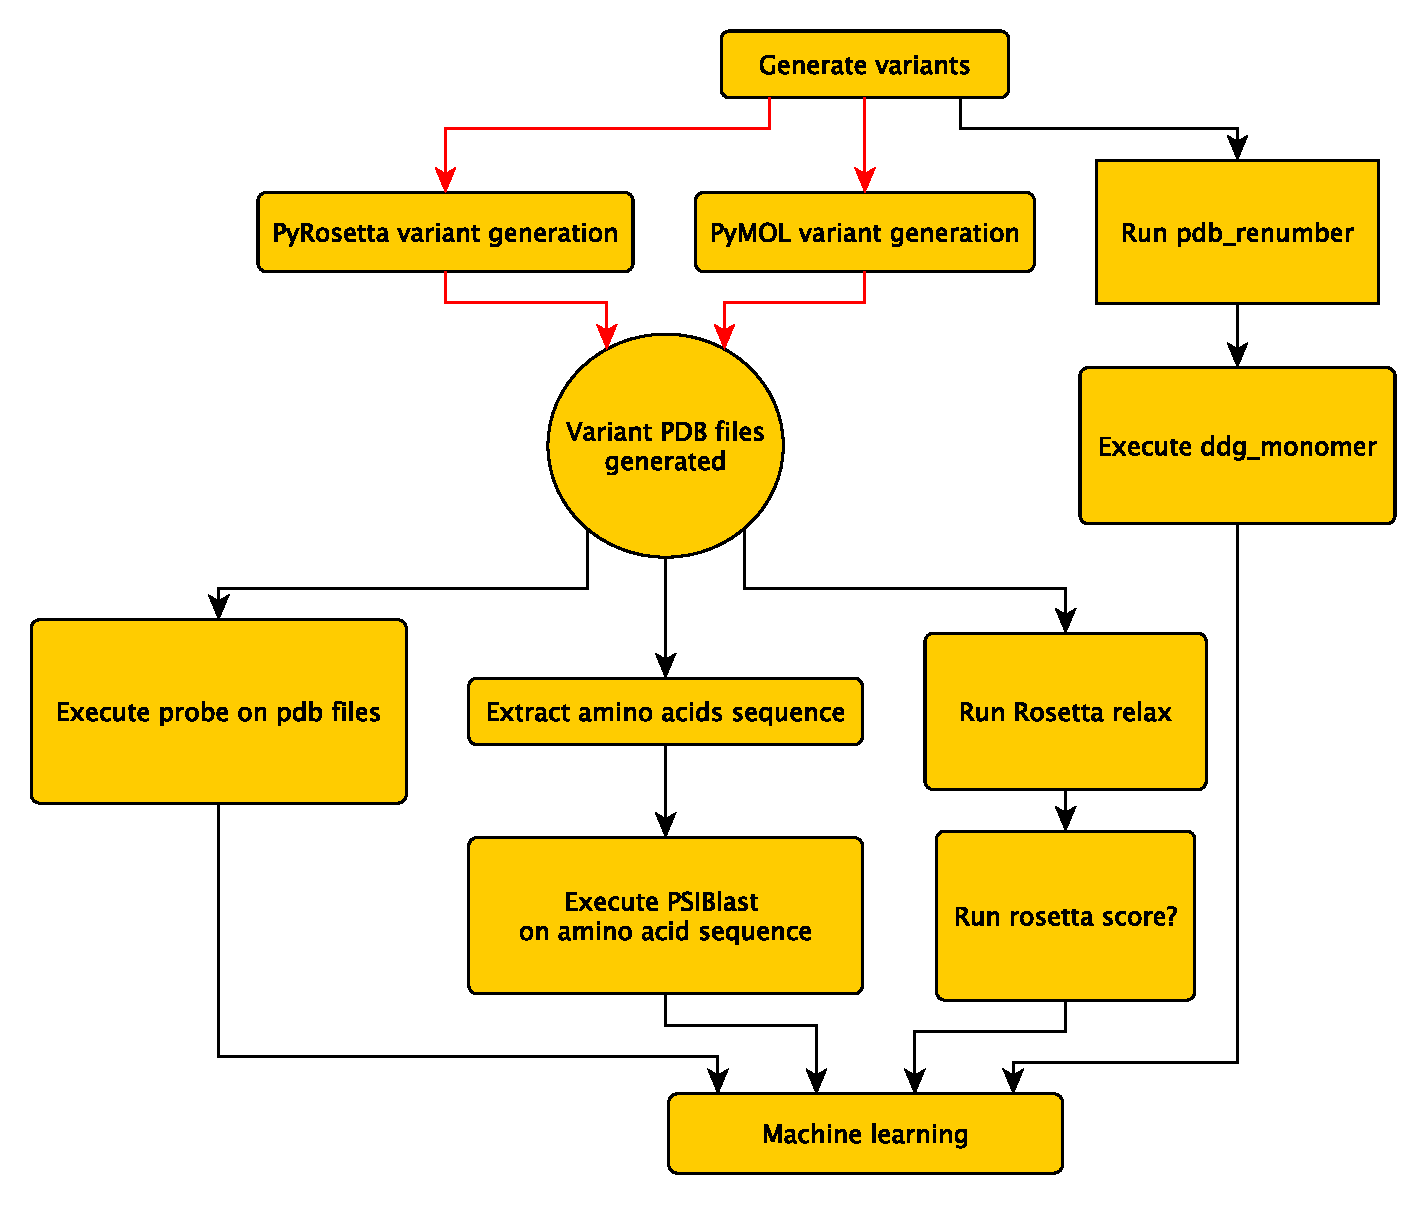
\includegraphics[width=\textwidth]{Flowcharts/VIPUR_approach.pdf}{a}
			\phantomcaption
			\label{fig:RES_VIPUR_approach}
		\end{subfigure}
		\begin{subfigure}{0.45\textwidth}
			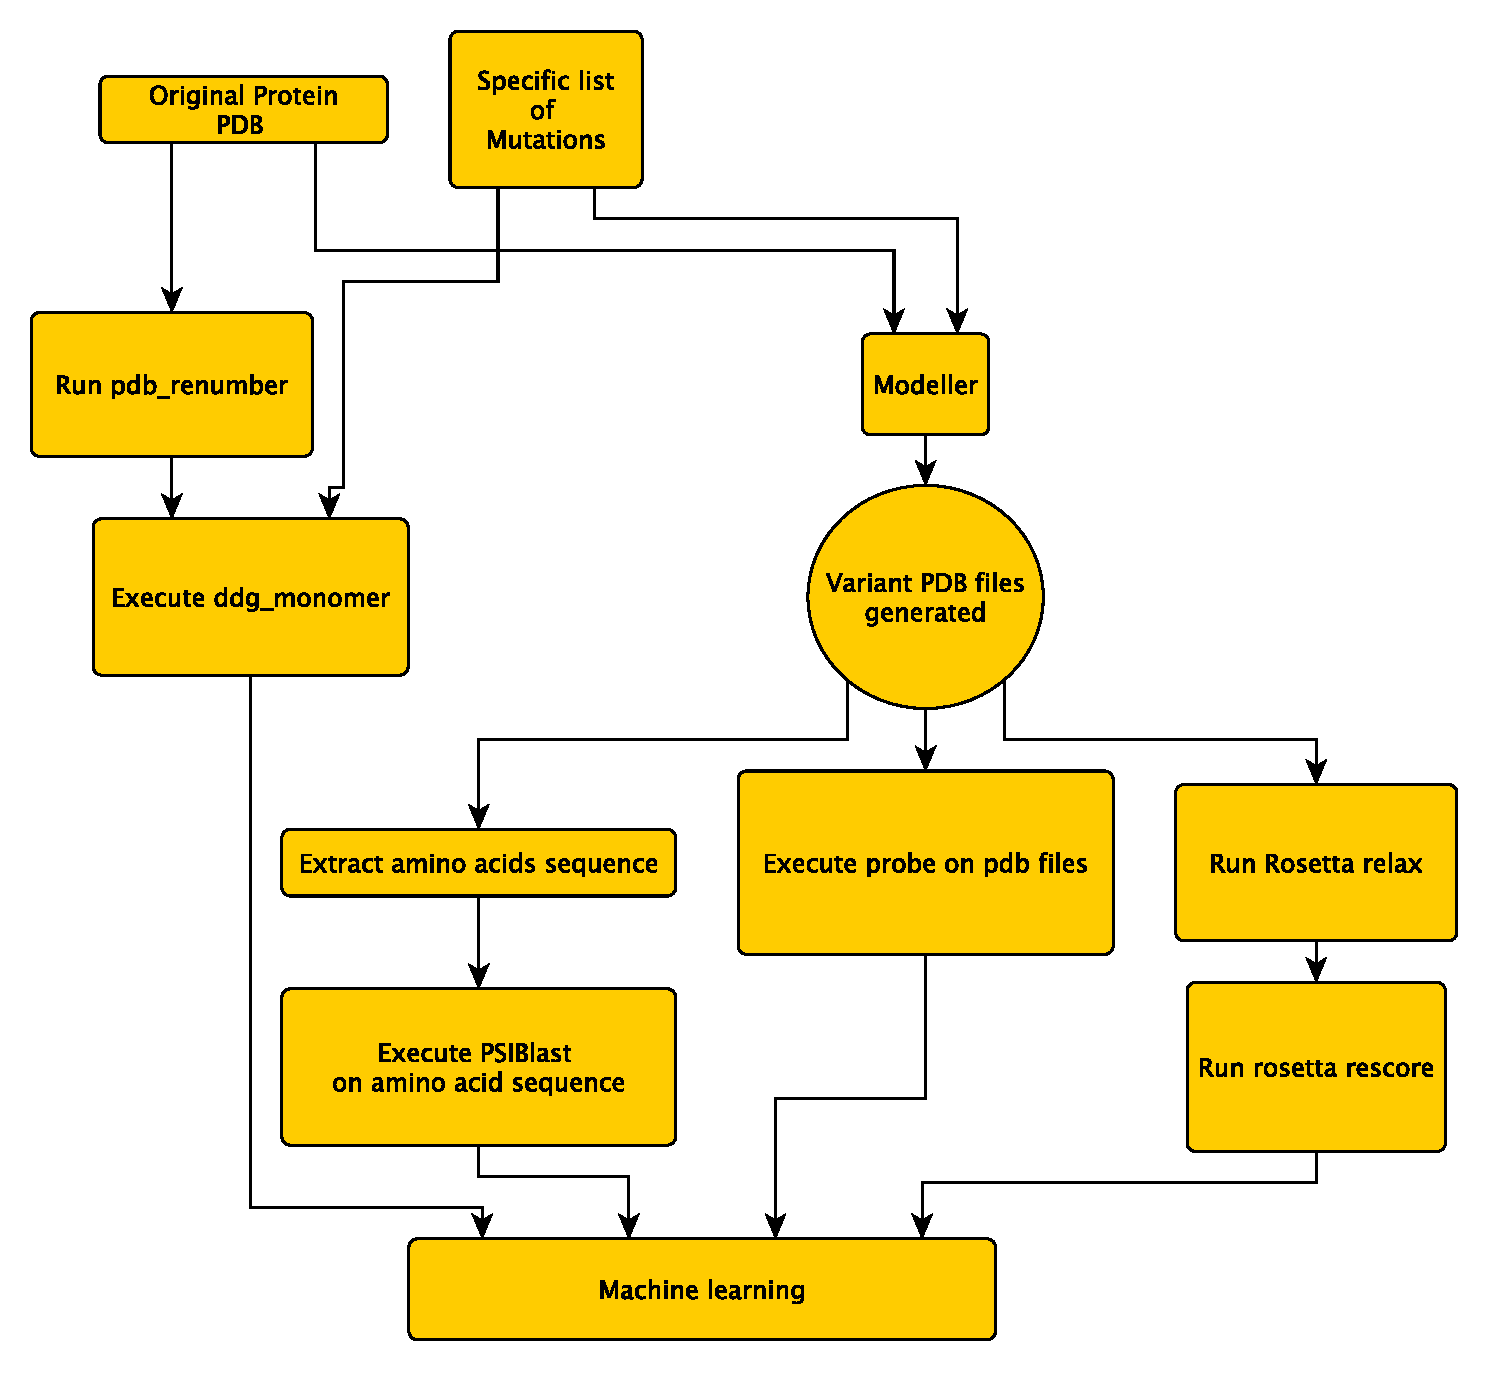
\includegraphics[width=\textwidth]{Flowcharts/Altered_VIPUR_approach.pdf}{b}
			\phantomcaption
			\label{fig:RES_Altered_VIPUR_approach}
		\end{subfigure}
		\caption[Flowcharts VIPUR pipeline and altered VIPUR pipeline]{Both flowcharts illustrate the VIPUR pipeline wherein each block is a procedure the central circle is the purpose of the mutated applications and each arrow represents the path to it. Figure \ref{fig:RES_VIPUR_approach} has red arrows that indicate that both methods were incapable to produce the mutated PDB files. Within figure \ref{fig:RES_Altered_VIPUR_approach} the alternative method is proposed wherein PyMOL and PyRosetta (Sections \ref{subsec:MM_PyMOL}, \ref{subsec:MM_PyRosetta}) is substituted by Modeller (Section \ref{subsec:MM_Modeller}) to acquire the mutated protein structures.}

		\label{fig:Flowcharts_of_old_and_altered_VIPUR}
	\end{figure}
	\label{subsubsec:RES_Incompatibility}
	\newpage
	
	\subsubsection{Expanding the VIPUR training set with data from TNFRSF1A by homology modeling and protein threading}
	Since the VTS did not have any features of TNFRSF1A (Section \ref{subsec:CD_TNFRSF1A}) the amino acid sequence was collected from Uniprot (Section \ref{subsec:MM_Uniprot}) and the protein from RCSB (Section \ref{subsec:MM_RCSB}). The structures available of TNFRSF1A were incomplete, fragments for the TNF $\alpha$ and $\beta$ binding site \cite{} were available and its death domain that interacts with TRADD \cite{} which plays a role in apoptosis (Section \ref{subsec:CD_TNFRSF1A}). To acquire a monomeric structure of TNFRSF1A two ab initio modeling web services I-TASSER and Robetta (Sections \ref{subsec:MM_I_TASSER}, \ref{subsec:MM_Robetta}) had been employed. Both were given the task to model the whole protein with and without a template to determine how well they could model a known structure and what it would form. Determination of which the best model was is based on the shortest distance ,defined root mean square deviation (RMSD), between a produced model compared to the X-ray crystallographic model of the TNFRSF1A binding site .
	
%	Solution structure of the tumor necrosis factor receptor-1 death domain, Sukits
	\begin{figure}[!ht]
		\centering
		\begin{subfigure}{0.45\textwidth}
			\includegraphics[width=\textwidth]{I_TASSER_Robetta_Images/1_EXT_ALIGN_I_TAS_WITHOUT_TEMPLATE.png}{a}
			\caption{RMSD = 28.786}
			\label{fig:RES_I_TASSER_Without}
		\end{subfigure}
		\begin{subfigure}{0.45\textwidth}
			\includegraphics[width=\textwidth]{I_TASSER_Robetta_Images/1_EXT_ALIGN_I_TAS_WITH_TEMPLATE.png}{b}
			\caption{RMSD =  3.830}
			\label{fig:RES_I_TASSER_With}
		\end{subfigure}
		\begin{subfigure}{0.45\textwidth}
			\includegraphics[width=\textwidth]{I_TASSER_Robetta_Images/1_EXT_ALIGN_ROB_WITHOUT_TEMPLATE.png}{c}
			\caption{RMSD =  3.067}
			\label{fig:RES_Robetta_Without}
		\end{subfigure}
		\begin{subfigure}{0.45\textwidth}
			\includegraphics[width=\textwidth]{I_TASSER_Robetta_Images/1_EXT_ALIGN_ROB_WITH_TEMPLATE.png}{d}
			\caption{RMSD =  2.877}
			\label{fig:RES_Robetta_With}
		\end{subfigure}
		\caption[I-TASSER and Robetta models with and without templates]{3D structures of TNFRSF1A ( \ref{fig:RES_I_TASSER_Without}, \ref{fig:RES_I_TASSER_With}: I-TASSER, \ref{fig:RES_Robetta_Without}, \ref{fig:RES_Robetta_With}: Robetta) without (left: \ref{fig:RES_I_TASSER_Without}, \ref{fig:RES_Robetta_Without}) and with templates (right: \ref{fig:RES_I_TASSER_With}, \ref{fig:RES_Robetta_With}). The sky blue colored structure in each figure is an X-ray crystallographic model (1EXT) of the binding site of TNFRSF1A and the orange structure is the representation of that identical fragment in the model made by the web services.}
	\end{figure}
	\label{subsubsec:RES_Expanding_Models}

\newpage
\subsection{Analyses of proteins variants TNFRSF1A}
	\subsubsection{Requirements for determining structural and binding effects of protein variants}
	Currently there is no protocol available to asses protein variants with structural information, 
	
	Assessing protein variants and its effects can be the most informative when assessed from multiple fields of view, however this is out of scope for this project and to simplify the problem it brought down to the perspective of function an form.
	
	Function determines how certain parts of the protein behave within an environment and determine its effects on a pathway. In context with TNFRSF1A one part resides on the cell surface where it binds ligands and on the cytoplasmic side it can interact with protein that triggers an inflammatory response or apoptosis. When a mutation is introduced at the cell surface side it might not be able to form dimer formations that interact with TNF ligands or during transformation with the binding of TNF it is unable to bind trimers. 
	
	Wherein the perspective of form the deciding factors are the amino acid sequence and where it resides within the cell.
	
	A different perspective is form wherein the amino acid sequence determines how a protein structure will be formed.
	
%	Assessing protein variants and its effects should be studied with a multidisciplinary view wherein form and function are assessed. Within the aspect of form should be seen how a protein is formed
%	
%	
%	However due to difficulties with experiments it can be hard to unravel all the effects that can be caused by mutations.
%	
%	 A part of this view is to know what function the protein has before its mutated to determine its effect on a pathway or function. 
%	
%	How does the 
%	
%	
%%	 Effect
%	Can a cell or pathway still function without this protein? or is there an alternative mechanism within the cell that is less efficient in performing similar role? 
	
	\subsubsection{Tools for assessing protein variant mutation}
	Before introducing mutations it is helpful to know if they are observed since not every mutation has the same occurrence, therefore three tables with observed TNFRSF1A mutations(Sections \ref{subsec:MM_GAVIN_data_table}, \ref{subsec:MM_GnomAD}, \ref{subsec:MM_Infevers}) have been combined into a single table consisting of two columns. The first column contains strings that describe the: original residue, position and where the residue is mutated to, the second column describes the observed effect of the mutation.	
	\begin{table}[ht]
		\begin{tabular}{ l | l | l | l}
			Original residue & Position in the protein sequence & New residue & Classification\\ \hline
			Cys & 44 & Tyr & PATHOGENIC\\
			Thr & 44 & Pro & PATHOGENIC\\
			Thr & 44 & Ser & PATHOGENIC\\
		\end{tabular}
		\caption[Sample of combined tables with observed mutations]{The format wherein mutations were filtered from the GAVIN, GenomAD and Infevers tables (Sections \ref{subsec:MM_GAVIN_data_table},  \ref{subsec:MM_GenomAD}, \ref{subsec:MM_Infevers}), the first column is split into original residue within a structure the position where it resides in amino acid sequence and the residue where it is altered to.  In the last part with the available classifications: Benign Pathogenic, Likely Benign, Likely Pathogenic, Population, Uncertain significance (VOUS) and Na. To see the whole table visit the supplementary.}
		\label{table:Res_Filtered_Mutations}
	\end{table}
	
%	the function of the mutated protein is within a pathway 
%	A broad perspective should be taken with a 
%	To determine the effects of mutated residue awithin a protein variant a b than structural information should
%	Up until VIPUR and the development of similar approaches that benefit from structural information
%VIPUR: Variant Interpretation and Prediction Using Rosetta, Baugh



%Something about that we tried to use the VTS and add our protein for information.

%
%\begin{table}[ht]
%	\begin{tabular}{ l | l | l | l | l}
%		Iteration number & Filename & Chain & Residue index in chain & New residue\\ \hline
%		34 & 1tnr3\_TNFA & R & 0 & TYR\\
%		34 & 1tnr3\_TNFA & T & 0 & TYR\\
%		34 & 1tnr3\_TNFA & S & 0 & TYR\\
%		35 & 1tnr3\_TNFA & R & 0 & PRO\\
%		35 & 1tnr3\_TNFA & T & 0 & PRO\\
%		35 & 1tnr3\_TNFA & S & 0 & PRO\\
%		36 & 1tnr3\_TNFA & R & 0 & SER\\
%		36 & 1tnr3\_TNFA & T & 0 & SER\\
%		36 & 1tnr3\_TNFA & S & 0 & SER\\
%	\end{tabular}
%	\caption{The format that describes the mutations that should be made by Modeller (Section \ref{subsec:MM_Modeller}). The iteration number states if a mutation must be made in a single variant or in a different protein. Filename describes the protein to which the mutations are applied. Since structures can consist of multiple chains it has to be specified together with the index starting at 0 instead of 1 and finally to which residue it will be transformed.}
%		\label{table:Res_Modeller_Mutation_Format}
%\end{table}


	\label{section:Chap_Results}
	\newpage
	
	\section{Discussion}
	
People with rare diseases are hard to diagnose

Prediction of pathogenicity in variants momentarily done based on sequence information and has been successful for certain groups of genes \cite{}.
%GAVIN: Gene-Aware Variant INterpretation for medical sequencing, van der Velde
However pathogenticy of some genes with their variants cannot be classified by the currently used features for classification. Recently a method, called VIPUR, surfaced that incorporated sequence and protein data for classification of the pathogenicity from gene variants\cite{}. 
%Robust classification of protein variation using structural modelling and large-scale data integration, Baugh

In the attempt to reproduce the methods taken by the VIPUR approach on protein structures that are related to rare diseases it was realized that some questionable steps were being taken. With this approach all ligands were removed \cite{} which changes the energies within and can therefor alter the structure \cite{} and causes it to be analyzed from a single perspective instead of two when a bound ligand is also taken into account. 
%Robust classification of protein variation using structural modelling and large-scale data integration, Baugh
%Application of a Theory of Enzyme Specificity to Protein Synthesis*, Koshland
Another step that was taken with VIPUR is that each structure is viewed as a monomer which is for some proteins not a problem, but for a complex that consists of multiple similar or a variety of different monomers makes it difficult to assess the effects.

To make predictions for new benign and pathogenic variants from TNFRSF1A, more information should be collected on how certain residues contribute to TNFRSF1A. More differences between interaction energies in mutated proteins could have been found be by adding molecular dynamics (MD) simulations of TNF $\alpha$/$\beta$ separately TNFRSF1A and combined with TNF docked into TNFRSF1A.



 prediction of potential benign and pathogenic variants of TNFRSF1A isoforms should be included in the analysis to gain insight in which part of the proteins are highly important for the interactions and could result in a better prediction.

 A significant contribution to gain more insight in how TNFRSF1A interacts with TNF $\alpha$/$\beta$ would have been the addition of molecular dynamic simulations; it shows how the proteins move on their own but also how the residues of the protein and the ligand interact with each other.



Isoforms were not taken into account.



 some steps have become questionable in structure of TNFRSF1A some questionable  rare diseases  some questionable  training set some q to reproduce some of the results that were acquired with the VIPUR some questionable assu


Looking at the investigation t

With the resource at our disposal we were unable to reproduce any of the results that were produced by VIPUR for testing purposes, by 
	\label{section:Chap_Discussion}
	\newpage
	
	\section{Conclusion}
	While VIPUR might be missing information to give a solid prediction about the pathogenicty of a protein variant, the detailed method used for determining the changes in energy levels could be a more reliable source for making predictions based of features.

 of info that accurate we propsed another method for assessing protein structures within complex which may play a role in machine learning
	\label{section:Chap_Conclusion}
	\section{Future work}
	The VIPUR approach will be further investigated to test whether the features generated by PSI-BLAST are the main predictors. To measure PSI-BLAST feature importance within VIPUR it first needs to be reverse engineered to make it work with Modeller or another tool which is able to implement mutations in PDB files. Once the reverse engineering is finished VIPURs feature importance is tested with shap\cite{} and or similar methods and software on the VTS.
%slundberg/shap: A unified approach to explain the output of any machine learning model, Slundberg
%Explaining Prediction Models and Individual Predictions with Feature Contributions, Štrumbelj
%Why Should I Trust You?": Explaining the Predictions of Any Classifier, Ribeiro
%Learning Important Features Through Propagating Activation Differences, Shrikumar
%Algorithmic Transparency via Quantitative Input Influence: Theory and Experiments with Learning Systems, Datta
%On Pixel-Wise Explanations for Non-Linear Classifier Decisions by Layer-Wise Relevance Propagation, Bach
%Interpreting random forests | Diving into data, Datadive

Currently SPVAA is not an automated method to predict pathogencity or deleteriouness of proteins, to transform it into an automated method the approach described in section \ref{subsec:GD_theoratical_large_scale_implementation} would be its guideline. 


%However it is at its current state it is a pipeline instead of a automated prediction tool that classifies protein variants. 

At the moment when its 


The cluster on which it is build does not optimal ran does not suffice to predict 
SPVAA is not feasible on the current cluster due to the lack of nodes and support for multi-node jobs which in both influence the amount of structures produced and therefore affect prediction accuracy. Two options are possible to improve the and has to use different software which is less resource intensive for predicting protein structures or it should only be used on larger clusters which have more nodes and support multi-node jobs. 




	\label{section:Chap_Future_Work}
	\newpage
	
	
	\printbibliography
	\newpage
	
	\section*{Supplementary}
	\begin{longtable}[l]{l|l}
	Mutation & Classification\\ \hline
	Ser4Phe & NA \\
	Val6Met & NA \\
	Pro7Thr & NA \\
	Pro12Leu & NA \\
	Glu14Lys & PATHOGENIC \\
	Leu15Val & NA \\
	Thr16Pro & PATHOGENIC \\
	Thr16Ala & PATHOGENIC \\
	Cys17Ser & PATHOGENIC \\
	Val20Ala & Uncertain significance (VOUS) \\
	Val21Ile & PATHOGENIC \\
	Gly21Ala & NA \\
	Val21Phe & PATHOGENIC \\
	Val21Leu & PATHOGENIC \\
	Arg24Trp & BENIGN \\
	Gly26Ala & NA \\
	Val27Asp & NA \\
	Ile28Phe & NA \\
	Arg28Trp & PATHOGENIC \\
	Ala30Pro & PATHOGENIC \\
	Ala30Gly & PATHOGENIC \\
	Ala30Ser & PATHOGENIC \\
	Ala30Thr & PATHOGENIC \\
	Val31Gly & NA \\
	Val33Leu & PATHOGENIC \\
	Val33Met & PATHOGENIC \\
	Arg34Thr & PATHOGENIC \\
	Gly35Arg & NA \\
	Ser38Pro & PATHOGENIC \\
	Pro39Thr & PATHOGENIC \\
	Asp41His & NA \\
	Asp41Glu & NA \\
	Thr43Ser & PATHOGENIC \\
	Cys44Tyr & PATHOGENIC \\
	Thr44Pro & PATHOGENIC \\
	Thr44Ser & PATHOGENIC \\
	Ser45Pro & PATHOGENIC \\
	Ala48Thr & PATHOGENIC \\
	Tyr49His & PATHOGENIC \\
	Tyr49Cys & PATHOGENIC \\
	Tyr49Asp & PATHOGENIC \\
	Ala50Thr & POPULATION \\
	Ile50Val & NA \\
	His51Arg & PATHOGENIC \\
	His51Tyr & PATHOGENIC \\
	Ala51Gly & PATHOGENIC \\
	Ala51Pro & PATHOGENIC \\
	His51Gln & Likely pathogenic \\
	Pro52Ala & PATHOGENIC \\
	Asn54Asp & Uncertain significance (VOUS) \\
	Ala54Thr & PATHOGENIC \\
	Glu55Lys & PATHOGENIC \\
	Ser56Thr & NA \\
	Ser56Leu & NA \\
	Ile57Ser & Uncertain significance (VOUS) \\
	Cys58Ser & PATHOGENIC \\
	Cys58Gly & PATHOGENIC \\
	Cys58Phe & PATHOGENIC \\
	Cys58Trp & Likely pathogenic \\
	Cys58Tyr & PATHOGENIC \\
	Cys58Arg & PATHOGENIC \\
	Cys59Tyr & PATHOGENIC \\
	Cys59Ser & NA \\
	Cys59Arg & PATHOGENIC \\
	Cys59Phe & PATHOGENIC \\
	Cys62Tyr & PATHOGENIC \\
	Cys62Gly & PATHOGENIC \\
	Gly65Glu & PATHOGENIC \\
	Pro66Arg & POPULATION \\
	Ala66Thr & PATHOGENIC \\
	Pro66Leu & BENIGN \\
	Thr66Ile & Likely pathogenic \\
	Tyr67Ser & PATHOGENIC \\
	Tyr67Cys & PATHOGENIC \\
	Pro68Leu & POPULATION \\
	Leu68Phe & PATHOGENIC \\
	Leu70Ser & POPULATION \\
	Gly70Arg & PATHOGENIC \\
	Thr70Met & PATHOGENIC \\
	Asp71Glu & Likely pathogenic \\
	Ser72Pro & PATHOGENIC \\
	Cys72Gly & Pathogenic \\
	Glu72Gly & POPULATION \\
	Cys72Tyr & PATHOGENIC \\
	Cys72Phe & PATHOGENIC \\
	Cys72Arg & PATHOGENIC \\
	Cys72Trp & PATHOGENIC \\
	Cys72Ser & PATHOGENIC \\
	Pro72Ser & POPULATION \\
	Pro73Ser & NA \\
	Cys73Arg & POPULATION \\
	Cys74Arg & PATHOGENIC \\
	Val74Gly & PATHOGENIC \\
	Val74Met & PATHOGENIC \\
	Val74Leu & PATHOGENIC \\
	Cys74Tyr & PATHOGENIC \\
	Cys75Arg & PATHOGENIC \\
	Cys75Tyr & PATHOGENIC \\
	Cys75Ser & PATHOGENIC \\
	Thr75Ala & PATHOGENIC \\
	Pro75Leu & NA \\
	Pro75Arg & NA \\
	Ala75Thr & POPULATION \\
	Ala76Thr & PATHOGENIC \\
	Glu76Asp & PATHOGENIC \\
	Arg78Pro & PATHOGENIC \\
	Thr79Met & PATHOGENIC \\
	Ser79Pro & PATHOGENIC \\
	Thr79Lys & Likely pathogenic \\
	Phe80Ser & PATHOGENIC \\
	Phe80Leu & PATHOGENIC \\
	Thr80Ile & POPULATION \\
	Phe80Val & PATHOGENIC \\
	Cys81Ser & PATHOGENIC \\
	Thr81Asn & PATHOGENIC \\
	Val81Ala & POPULATION \\
	Cys81Arg & PATHOGENIC \\
	Cys81Trp & PATHOGENIC \\
	Cys81Tyr & PATHOGENIC \\
	Cys81Phe & PATHOGENIC \\
	Arg82Gly & Uncertain significance (VOUS) \\
	Cys82Trp & PATHOGENIC \\
	Cys82Phe & PATHOGENIC \\
	Cys82Tyr & PATHOGENIC \\
	Gly83Asp & POPULATION \\
	Cys84Arg & PATHOGENIC \\
	Cys84Tyr & PATHOGENIC \\
	Cys84Ser & PATHOGENIC \\
	Glu85Asp & NA \\
	Asn85Lys & PATHOGENIC \\
	Asn85Ile & PATHOGENIC \\
	His86Pro & PATHOGENIC \\
	His86Tyr & PATHOGENIC \\
	His86Leu & PATHOGENIC \\
	Leu87Pro & PATHOGENIC \\
	Leu87Phe & POPULATION \\
	Lys87Glu & POPULATION \\
	Gly87Ser & NA \\
	Gln88Glu & POPULATION \\
	Ser88Pro & PATHOGENIC \\
	Phe89Ser & PATHOGENIC \\
	Phe89Leu & PATHOGENIC \\
	Phe89Val & PATHOGENIC \\
	Cys90Ser & PATHOGENIC \\
	Cys90Gly & PATHOGENIC \\
	Cys90Tyr & PATHOGENIC \\
	Ser90Ala & PATHOGENIC \\
	Thr90Asn & PATHOGENIC \\
	Thr90Ile & NA \\
	Thr90Pro & NA \\
	Arg90Trp & POPULATION \\
	Ser90Pro & PATHOGENIC \\
	Cys90Arg & PATHOGENIC \\
	Tyr92His & POPULATION \\
	Ser92Asn & POPULATION \\
	Cys93Trp & PATHOGENIC \\
	Cys93Ser & PATHOGENIC \\
	Cys93Arg & PATHOGENIC \\
	Asn94Lys & PATHOGENIC \\
	Ser94Cys & PATHOGENIC \\
	Ser94Gly & POPULATION \\
	Asn94Ile & PATHOGENIC \\
	His95Pro & PATHOGENIC \\
	His95Leu & PATHOGENIC \\
	Ala95Thr & POPULATION \\
	Glu95Gly & POPULATION \\
	His95Tyr & NA \\
	Leu96Phe & POPULATION \\
	Leu96Pro & PATHOGENIC \\
	Cys96Tyr & PATHOGENIC \\
	Arg97Gln & PATHOGENIC \\
	Phe98Leu & PATHOGENIC \\
	Phe98Cys & PATHOGENIC \\
	His98Asn & NA \\
	Phe98Ile & PATHOGENIC \\
	Phe98Ser & PATHOGENIC \\
	Cys99Arg & PATHOGENIC \\
	Cys99Ser & PATHOGENIC \\
	Cys99Tyr & PATHOGENIC \\
	Cys99Gly & PATHOGENIC \\
	Cys100Arg & PATHOGENIC \\
	Ser101Asn & POPULATION \\
	Pro102Ser & POPULATION \\
	Asn102Asp & POPULATION \\
	Cys102Arg & PATHOGENIC \\
	Cys102Ser & PATHOGENIC \\
	Cys102Trp & PATHOGENIC \\
	Cys103Tyr & POPULATION \\
	Ser103Cys & PATHOGENIC \\
	Cys105Tyr & PATHOGENIC \\
	Arg106Gln & PATHOGENIC \\
	Ser106Pro & PATHOGENIC \\
	Leu107Phe & POPULATION \\
	Cys108Arg & PATHOGENIC \\
	Cys108Tyr & PATHOGENIC \\
	Thr109Ala & PATHOGENIC \\
	Thr110Ile & POPULATION \\
	Val111Leu & POPULATION \\
	Gln111Lys & Uncertain significance (VOUS) \\
	Arg112Pro & PATHOGENIC \\
	Val112Leu & Likely pathogenic \\
	His112Tyr & PATHOGENIC \\
	Val112Met & NA \\
	Leu113Phe & POPULATION \\
	Thr114Ile & POPULATION \\
	Ile114Ser & NA \\
	Val115Ala & POPULATION \\
	Ser115Pro & PATHOGENIC \\
	Ser115Phe & NA \\
	Cys116Tyr & PATHOGENIC \\
	Cys116Phe & PATHOGENIC \\
	Cys116Trp & PATHOGENIC \\
	Cys117Tyr & PATHOGENIC \\
	Cys117Arg & PATHOGENIC \\
	Gly117Asp & POPULATION \\
	Cys117Ser & Likely pathogenic \\
	Cys118Tyr & PATHOGENIC \\
	Thr118Ala & PATHOGENIC \\
	Met118Val & POPULATION \\
	Cys118Arg & PATHOGENIC \\
	Val119Gly & NA \\
	Val119Ala & NA \\
	Arg121Trp & Likely pathogenic \\
	Ser121Cys & POPULATION \\
	Arg121Pro & NA \\
	Arg121Gln & NA \\
	Arg121Gly & NA \\
	Asp122His & Likely pathogenic \\
	Asp122Glu & Uncertain significance (VOUS) \\
	Thr123Ile & NA \\
	Val124Gly & NA \\
	Val124Ala & NA \\
	Val124Met & NA \\
	Cys125Arg & Likely pathogenic \\
	Cys125Trp & PATHOGENIC \\
	Cys125Tyr & PATHOGENIC \\
	Cys125Phe & PATHOGENIC \\
	Gly126Asp & POPULATION \\
	His126Arg & POPULATION \\
	His126Tyr & POPULATION \\
	Cys127Tyr & PATHOGENIC \\
	Cys127Arg & PATHOGENIC \\
	Phe129Leu & POPULATION \\
	Asn130Lys & Likely pathogenic \\
	Gln131Glu & NA \\
	Arg133Trp & NA \\
	Arg133Gln & NA \\
	His134Pro & Uncertain significance (VOUS) \\
	Tyr135His & NA \\
	Glu135Val & POPULATION \\
	Tyr135Cys & Likely pathogenic \\
	Ser137Gly & NA \\
	Glu138Gly & NA \\
	Glu138Ala & Likely benign \\
	Ser140Thr & POPULATION \\
	Phe141Leu & PATHOGENIC \\
	Phe141Ser & PATHOGENIC \\
	Phe141Cys & PATHOGENIC \\
	Phe141Ile & PATHOGENIC \\
	Cys142Phe & POPULATION \\
	Cys143Trp & Likely pathogenic \\
	Cys143Arg & PATHOGENIC \\
	Ser145Asn & POPULATION \\
	Asn145Asp & NA \\
	Asn145Ser & NA \\
	Cys146Tyr & NA \\
	Leu150Phe & POPULATION \\
	Asn151Ser & NA \\
	Gly152Ala & NA \\
	Thr153Ile & POPULATION \\
	Leu153Val & POPULATION \\
	Val154Met & NA \\
	Val154Leu & NA \\
	His155Tyr & PATHOGENIC \\
	Ile156Asn & PATHOGENIC \\
	Leu156Phe & POPULATION \\
	Val159Asp & PATHOGENIC \\
	Arg160His & NA \\
	Arg160Leu & NA \\
	Arg160Ser & NA \\
	Arg160Cys & NA \\
	Lys161Arg & NA \\
	Ser162Cys & NA \\
	Ser162Ala & NA \\
	Pro163Ser & NA \\
	Asp164Asn & POPULATION \\
	Glu164Lys & NA \\
	Pro167Leu & NA \\
	Pro167Ala & NA \\
	Ser168Ala & NA \\
	Pro169Thr & NA \\
	His169Arg & NA \\
	His169Tyr & NA \\
	Pro169His & NA \\
	His170Tyr & NA \\
	Pro171Arg & NA \\
	Phe172Leu & NA \\
	Pro177Ser & NA \\
	Glu178Val & NA \\
	Glu178Lys & NA \\
	Ala179Thr & NA \\
	Ala179Ser & NA \\
	Ala179Glu & NA \\
	Ala179Val & NA \\
	Leu182Val & NA \\
	Ser183Thr & NA \\
	Leu185Arg & NA \\
	Cys185Phe & POPULATION \\
	Pro186Ser & NA \\
	Phe186Leu & BENIGN \\
	Pro187His & NA \\
	Pro187Leu & NA \\
	Pro187Ala & NA \\
	Ser188Asn & NA \\
	Arg189Cys & NA \\
	Glu190Lys & NA \\
	Phe190Leu & NA \\
	Phe190Val & NA \\
	Gly191Asp & NA \\
	Thr192Met & NA \\
	Leu196Val & NA \\
	Leu198Val & NA \\
	Ile199Asn & PATHOGENIC \\
	Ile199Thr & NA \\
	Arg201Ser & NA \\
	Arg201Cys & NA \\
	Arg201Gly & NA \\
	Arg201His & NA \\
	Val202Asp & PATHOGENIC \\
	His203Asn & NA \\
	Thr205Asn & NA \\
	Glu206Asp & NA \\
	Asp207Asn & NA \\
	Arg207Cys & NA \\
	Arg207His & NA \\
	His208Leu & NA \\
	Phe209Tyr & NA \\
	Gly214Arg & NA \\
	Pro215Thr & NA \\
	Trp215Cys & NA \\
	Gly216Glu & NA \\
	Pro217Leu & NA \\
	Cys217Tyr & NA \\
	Arg218Lys & NA \\
	Arg219His & NA \\
	Arg219Leu & NA \\
	Arg219Cys & NA \\
	Phe220Ser & NA \\
	Phe220Leu & NA \\
	Leu222Phe & NA \\
	Phe222Ser & NA \\
	Ser226Cys & NA \\
	Ala226Thr & NA \\
	Phe229Leu & NA \\
	Ile230Val & NA \\
	Gly231Val & NA \\
	Met233Leu & NA \\
	Arg235His & NA \\
	Gln237Arg & NA \\
	Arg238Gln & NA \\
	Ser241Phe & NA \\
	His242Arg & POPULATION \\
	His242Tyr & POPULATION \\
	Phe245Leu & POPULATION \\
	Glu248Lys & NA \\
	Glu248Asp & NA \\
	Gly250Arg & NA \\
	Leu251Phe & NA \\
	Glu251Val & POPULATION \\
	Pro253Thr & NA \\
	Pro253Ala & NA \\
	Glu253Lys & NA \\
	Glu254Ala & NA \\
	Glu255Gln & NA \\
	Lys255Glu & NA \\
	Gly256Glu & NA \\
	Gly256Val & NA \\
	Gly257Ala & NA \\
	Gly257Arg & NA \\
	Ala257Pro & NA \\
	Ala257Val & NA \\
	Gly259Arg & NA \\
	Gly259Glu & NA \\
	Leu259Ile & NA \\
	Leu259Arg & NA \\
	Gly260Val & NA \\
	Thr262Ala & NA \\
	Pro266Thr & NA \\
	Pro266Ala & NA \\
	Leu267Val & NA \\
	Arg268Gln & NA \\
	Trp269Arg & NA \\
	Arg269Lys & BENIGN \\
	Asn270Lys & NA \\
	Asn270Asp & NA \\
	Pro271Ser & NA \\
	Pro271Ala & NA \\
	Ser272Gly & NA \\
	Phe273Leu & NA \\
	Ser274Gly & NA \\
	Gly274Arg & NA \\
	Pro275Ser & NA \\
	Gly277Glu & BENIGN \\
	Thr280Ser & NA \\
	Thr280Asn & NA \\
	Pro281Arg & NA \\
	Ser282Leu & NA \\
	Arg284His & NA \\
	Arg284Cys & NA \\
	Arg284Leu & NA \\
	Trp285Arg & NA \\
	Phe285Leu & NA \\
	Ser286Ile & NA \\
	Pro287Ala & NA \\
	Val288Leu & NA \\
	Trp288Ser & NA \\
	Val288Met & NA \\
	Pro289Leu & NA \\
	Ala289Thr & NA \\
	Ser290Arg & NA \\
	Phe293Leu & NA \\
	Pro293Arg & NA \\
	Trp295Cys & NA \\
	Ser296Thr & NA \\
	Arg298Gly & NA \\
	Thr298Ala & NA \\
	Pro301Ser & NA \\
	Pro301His & NA \\
	Gly302Ser & NA \\
	Cys304Ser & NA \\
	Pro305Arg & NA \\
	Asn306Lys & NA \\
	Pro310Leu & NA \\
	Pro310Ser & NA \\
	Arg311Cys & NA \\
	Arg311His & NA \\
	Arg312Lys & NA \\
	Glu313Lys & NA \\
	Glu313Gln & NA \\
	Ala315Thr & NA \\
	Pro317Ala & NA \\
	Tyr318Cys & NA \\
	Tyr318Phe & NA \\
	Gly320Arg & NA \\
	Gly320Glu & BENIGN \\
	Asp322Glu & NA \\
	Pro323Ser & NA \\
	Ile324Val & NA \\
	Ile324Asn & NA \\
	Ala326Ser & NA \\
	Leu329Phe & NA \\
	Ala330Thr & NA \\
	Ala330Val & NA \\
	Pro333Ser & NA \\
	Ile334Val & NA \\
	Pro335His & NA \\
	Pro335Arg & NA \\
	Asn336Lys & NA \\
	Asn336Asp & NA \\
	Leu338Phe & NA \\
	Lys340Arg & NA \\
	Lys340Glu & NA \\
	Glu342Asp & NA \\
	His346Arg & NA \\
	His346Gln & NA \\
	Thr353Ala & NA \\
	Thr353Pro & NA \\
	Pro356Ser & NA \\
	Pro356Ala & NA \\
	Thr358Ala & NA \\
	Glu364Val & NA \\
	Pro368Ser & NA \\
	Pro368Ala & NA \\
	Ser381Asn & NA \\
	Asp382His & NA \\
	His383Asn & NA \\
	Asp386Glu & NA \\
	Leu388Arg & NA \\
	Leu390Pro & NA \\
	Arg394His & NA \\
	Cys395Arg & NA \\
	Cys395Trp & NA \\
	Leu396Arg & NA \\
	Glu398Lys & NA \\
	Ser402Gly & NA \\
	Ala405Gly & NA \\
	Arg408Lys & NA \\
	Arg409Trp & NA \\
	Arg409Leu & NA \\
	Pro412Leu & NA \\
	Arg413Gly & NA \\
	Arg413Gln & NA \\
	Glu415Lys & NA \\
	Ala416Gly & NA \\
	Thr417Ala & NA \\
	Glu419Gly & NA \\
	Gly422Arg & NA \\
	Arg423His & NA \\
	Arg426His & NA \\
	Gly432Val & NA \\
	Glu435Gly & NA \\
	Asp436Gly & NA \\
	Glu438Lys & NA \\
	Glu438Ala & NA \\
	Glu438Gln & NA \\
	Cys442Tyr & NA \\
	Gly443Arg & NA \\
	Gly443Val & NA \\
	Pro448Leu & NA \\
	Ser452Gly & NA \\
	Leu453Pro & NA \\
\end{longtable}
\label{table:All_TNFR1_mutations}
\newpage
\input{Tables/RelevantTNFR1mutations}
\label{table:Relevant_TNFR1_mutations}
\newpage

	\label{section:Chap_Supplementary}
	\newpage
	

	
	
\end{document}